% بخش استنتاج هوشمند RAG برای گزارش اصلی

\section{سیستم استنتاج هوشمند RAG}
این بخش به تشریح سیستم استنتاج هوشمند \lr{RAG} می‌پردازد که با استفاده از \lr{LangGraph} برای تصمیم‌گیری خودکار و بهینه‌سازی فرایند بازیابی اطلاعات طراحی شده است. این سیستم قابلیت تشخیص زمان مناسب برای بازیابی اسناد و زمان پاسخ مستقیم را داراست و تجربه‌ای گفتگو محور و متناسب با بافت ارائه می‌دهد.

\noindent
مزایای کلیدی سیستم استنتاج هوشمند:
\begin{itemize}
    \item \textbf{تصمیم‌گیری هوشمند:} استفاده از مدل زبان بزرگ برای تشخیص نیاز به بازیابی اسناد یا پاسخ مستقیم
    \item \textbf{ارزیابی کیفیت اسناد:} بررسی مرتبط بودن اسناد بازیابی شده قبل از تولید پاسخ
    \item \textbf{بهبود پرس‌وجو:} بازنویسی خودکار سؤالاتی که نتایج مرتبط ارائه نمی‌دهند
    \item \textbf{بازیابی تصاویر:} دریافت خودکار تصاویر مرتبط هنگام وجود ارجاع تصویر در بخش‌های متن
    \item \textbf{مدیریت گفتگو:} حفظ وضعیت و بافت گفتگو در طول جلسات
\end{itemize}

\newpage

\section{معماری گردش کار استنتاج}

\begin{figure}[!htbp]
    \centering
    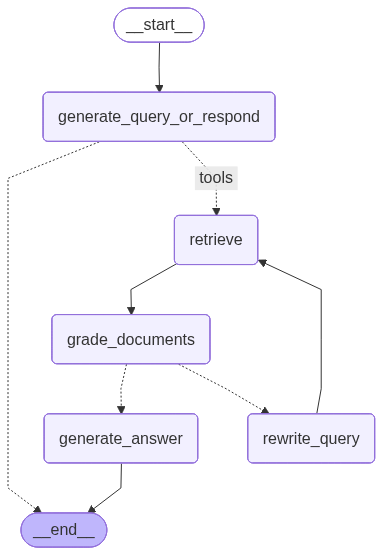
\includegraphics[width=0.65\textwidth]{agentic_rag_workflow.png}
    \caption{نمونه‌ای از گردش کار استنتاج هوشمند \lr{RAG}. این تصویر مراحل مختلف فرایند استنتاج را نشان می‌دهد، از جمله دریافت پرس‌وجو، تصمیم‌گیری برای بازیابی اسناد، و تولید پاسخ نهایی.}
    \label{fig:agentic_rag_workflow}
\end{figure}

\subsection{مراحل فرایند}
سیستم استنتاج هوشمند \lr{RAG} دارای گردش کار مبتنی بر گراف است که شامل مراحل زیر می‌باشد:

\subsection*{گره‌های اصلی}
\begin{itemize}
    \item \textbf{گره عامل (\lr{Agent Node}):} تصمیم‌گیری برای بازیابی اسناد یا پاسخ مستقیم
    \item \textbf{ابزار بازیابی (\lr{Retrieval Tool}):} جستجو برای اسناد مرتبط با استفاده از جستجوی ترکیبی
    \item \textbf{ارزیابی اسناد (\lr{Document Grading}):} بررسی میزان مرتبط بودن اسناد بازیابی شده
    \item \textbf{بازنویسی سؤال (\lr{Question Rewriting}):} بهبود سؤالاتی که نتایج مرتبط ارائه نمی‌دهند
    \item \textbf{تولید پاسخ (\lr{Answer Generation}):} تولید پاسخ نهایی با استفاده از بافت بازیابی شده
\end{itemize}

\subsection*{الگوریتم گردش کار}
فرایند تصمیم‌گیری سیستم به صورت زیر عمل می‌کند:

\begin{enumerate}
    \item \textbf{دریافت پرس‌وجوی کاربر:} سیستم پیام کاربر را دریافت و تحلیل می‌کند
    \item \textbf{تصمیم‌گیری اولیه:} عامل تصمیم می‌گیرد که آیا نیاز به بازیابی اسناد است یا می‌تواند مستقیماً پاسخ دهد
    \item \textbf{بازیابی شرطی:} در صورت نیاز، ابزار بازیابی فعال شده و اسناد مرتبط جستجو می‌شوند
    \item \textbf{ارزیابی کیفیت:} میزان مرتبط بودن اسناد بازیابی شده با پرس‌وجو ارزیابی می‌شود
    \item \textbf{حلقه بازخورد:} در صورت عدم مرتبط بودن، سؤال بازنویسی شده و فرایند تکرار می‌شود
\end{enumerate}


\subsection{فرایند تولید پاسخ}

\subsubsection*{حاشیه‌نویسی شناسه‌های بخش}
بخش‌های بازیابی شده به همراه شناسه‌های یکتای خود (\lr{chunk\_id}) به مدل زبان بزرگ ارسال می‌شوند. هر بخش با فرمت زیر حاشیه‌نویسی می‌شود(شکل \ref{fig:tool_response}).

این حاشیه‌نویسی به مدل زبان بزرگ اجازه می‌دهد تا دقیقاً مشخص کند کدام بخش‌ها در تولید پاسخ استفاده شده‌اند.

\begin{figure}[!htbp]
    \centering
    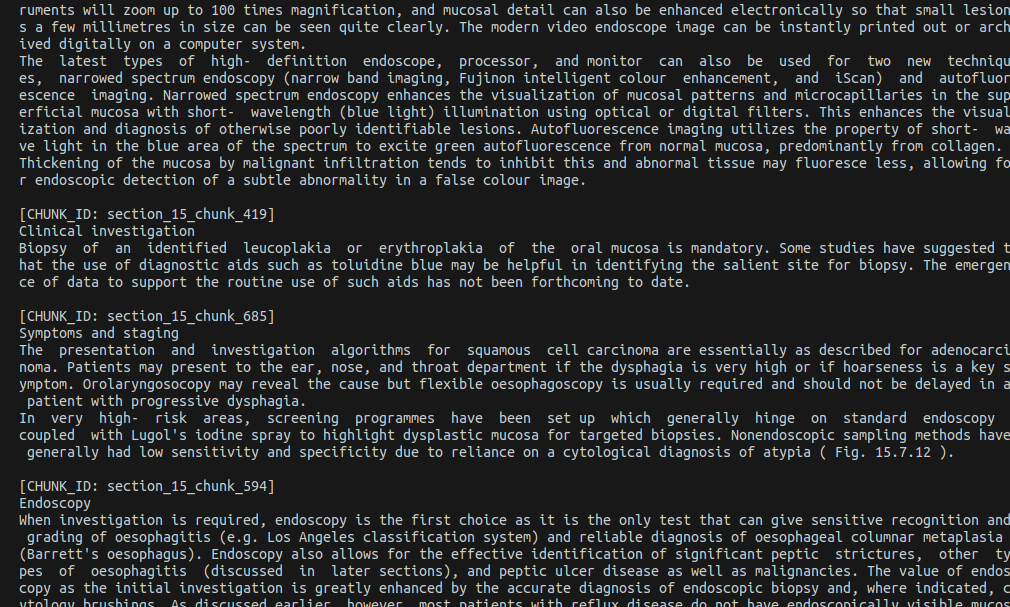
\includegraphics[width=0.95\textwidth]{tool_response.png}
    \caption{نمونه‌ای از پاسخ ابزار بازیابی که شامل بخش‌های حاشیه‌نویسی شده با شناسه‌های یکتا می‌باشد. این فرمت به مدل زبان بزرگ کمک می‌کند تا منابع استفاده شده را به دقت مشخص کند.}
    \label{fig:tool_response}
\end{figure}

\subsubsection*{تولید پاسخ ساختاریافته}
مدل زبان بزرگ پاسخی ساختاریافته تولید می‌کند که شامل دو بخش است:

\begin{itemize}
    \item \textbf{پاسخ (\lr{answer}):} متن پاسخ نهایی برای کاربر
    \item \textbf{شناسه‌های استفاده شده (\lr{chunk\_ids\_used}):} فهرست شناسه‌های بخش‌هایی که در تولید پاسخ مورد استفاده قرار گرفته‌اند
\end{itemize}

\noindent
نمونه‌ای از پاسخ ساختاریافته تولید شده توسط مدل:

\begin{latin}
\begin{verbatim}
{
  "answer": "Narrow band imaging, a type of narrowed 
  spectrum endoscopy, uses short-wavelength (blue light) 
  illumination with optical or digital filters. This 
  technique enhances the visualization of mucosal 
  patterns and microcapillaries in the superficial 
  mucosa, which helps in better visualizing and 
  diagnosing otherwise poorly identifiable lesions, 
  including distinguishing columnar from squamous mucosa.",
  "chunk_ids_used": [
    "section_15_chunk_101", 
    "section_15_chunk_620"
  ]
}
\end{verbatim}
\end{latin}

این ساختار به سیستم اجازه می‌دهد تا دقیقاً بخش‌های استفاده شده را شناسایی و متادیتای مرتبط را استخراج کند.

\subsection{استخراج متادیتا و بازیابی تصاویر}
پس از دریافت پاسخ از مدل زبان بزرگ، سیستم فرایند استخراج تصاویر مرتبط را آغاز می‌کند:

\subsubsection*{الگوریتم استخراج تصاویر}
\begin{enumerate}
    \item \textbf{شناسایی بخش‌های استفاده شده:} بر اساس \lr{chunk\_ids\_used}، اشیاء دقیق بخش‌ها از لیست بازیابی شده انتخاب می‌شوند
    \item \textbf{بررسی متادیتا:} برای هر بخش، فیلد \lr{meta.doc\_items} در متادیتا بررسی می‌شود
    \item \textbf{شناسایی تصاویر والد:} عناصری با برچسب \lr{"label": "picture"} شناسایی می‌شوند
    \item \textbf{استخراج شناسه تصویر:} از فیلد \lr{self\_ref} شناسه تصویر استخراج می‌شود
    \item \textbf{بازیابی تصویر کامل:} تصویر کامل به همراه توضیحات تولید شده توسط مدل چندوجهی از مخزن اسناد بازیابی می‌شود
    \item \textbf{الحاق به پاسخ:} تصاویر به پاسخ نهایی عامل الحاق می‌شوند
\end{enumerate}

این فرایند تضمین می‌کند که تمامی اطلاعات بصری مرتبط با پاسخ، به همراه متن، در اختیار کاربر قرار گیرد.

\subsection{پیاده‌سازی لایه رابط کاربری}
در لایه \lr{Framework}، یک ربات تلگرام پیاده‌سازی شده است که رابط کاربری تعاملی برای سیستم فراهم می‌آورد:

\subsubsection*{مدیریت بخش‌ها در ربات تلگرام}
\begin{enumerate}
    \item \textbf{ذخیره‌سازی بخش‌ها:} پس از دریافت پاسخ از عامل، بخش‌های استفاده شده در حافظه موقت ذخیره می‌شوند
    \item \textbf{تولید دکمه‌های تعاملی:} برای هر \lr{chunk\_id}، یک دکمه \lr{Inline Keyboard} در پیام تلگرام ایجاد می‌شود
    \item \textbf{پردازش کلیک کاربر:} هنگامی که کاربر روی دکمه شناسه بخش کلیک می‌کند، سیستم محتوای کامل بخش را از حافظه می‌خواند
    \item \textbf{نمایش جزئیات:} محتوای بخش به همراه متادیتای مرتبط برای کاربر نمایش داده می‌شود
\end{enumerate}

این رویکرد به کاربران اجازه می‌دهد تا شفافیت کاملی نسبت به منابع استفاده شده در تولید پاسخ داشته باشند و در صورت نیاز، محتوای اصلی بخش‌ها را مشاهده کنند.

\section{نتیجه‌گیری}
سیستم استنتاج هوشمند \lr{RAG} با استفاده از \lr{LangGraph} قابلیت‌های پیشرفته‌ای برای تصمیم‌گیری خودکار و بهینه‌سازی فرایند بازیابی اطلاعات فراهم می‌آورد. این رویکرد نه تنها کارایی سیستم را بهبود می‌بخشد بلکه تجربه کاربری بهتری نیز ارائه می‌دهد. ترکیب تصمیم‌گیری هوشمند، ارزیابی کیفیت اسناد، و بازنویسی پرس‌وجو منجر به سیستمی قدرتمند و انطباق‌پذیر شده است که می‌تواند در کاربردهای مختلف پردازش اسناد پزشکی مورد استفاده قرار گیرد.
